\documentclass[11pt,a4paper]{article}
\usepackage{jmlr2e}
\usepackage{a4wide}
\usepackage[utf8]{inputenc}
\usepackage[T2A]{fontenc}
\usepackage{graphics,graphicx,epsfig}
\let\proof\relax
\let\endproof\relax
\usepackage{amssymb,amsfonts,amsthm,amsmath,mathtext,enumerate,float}
\usepackage[russian,english]{babel}
\usepackage[all]{xy}
\usepackage{morefloats}
\usepackage{pgf}
\usepackage[debug,outputdir={docgraphs/}]{dot2texi}
\usepackage{tikz}
\usepackage{scalefnt}
\usepackage{listings}
\usepackage{float}
\usepackage{verbatim}
\usepackage{placeins}
\usepackage{url}
\usepackage{babelbib}
\usepackage{pbox}
\usepackage{grffile}
\usepackage{color}
\usepackage{xfrac}
\usepackage{comment}
\usepackage{rotating}
\usepackage{sectsty}
\usepackage{caption}
\usepackage{subcaption}
\usetikzlibrary{shapes,arrows}
\usetikzlibrary{decorations.pathmorphing}

% Comment the following block when compiling this .tex with a saner compiler than texlive.
\makeatletter
\def\@settitle{\begin{center}%
    \baselineskip14\p@\relax
    \bfseries
    \@title
  \end{center}%
}

\makeatother

\theoremstyle{definition}
\newtheorem{algo}{Алгоритм}
\newtheorem{stat}{Утверждение}
\newtheorem{defin}{Определение}
\newtheorem{note}{Замечание}

\begin{document}

\begin{center}
  STABILITY OF NON-LINEAR REGRESSION MODELS WITH RESPECT TO VARIATIONS IN THE MEASURED DATA

  \bigskip
  G.~Rudoy
\end{center}

\begin{abstract}
  A set of various non-linear regression models is considered to select an optimal one
  describing a given physical experiment.
  For this, a new model selection criteria is proposed, which we will call model \emph{stability}.
  This criteria shows the dependency of the model parameters on the variation of samples in
  the learning set.
  The proposed stability criteria is also used to estimate the error of determining the model
  parameters, which is of interest to the experts.
  Experimental data for refraction index of transparent polymers at different wavelengths is
  used as illustration of the criteria, studying several different expert-proposed models.
  The criteria is also illustrated for the case of a linear model, where a known theoretical
  estimate of parameters errors exists.

  \bigskip
  \textbf{Keywords}: \emph{symbolic regression, non-linear models, inductive generation,
	model stability, transparent polymers dispersion.}
\end{abstract}

\section*{Introduction}

Analysis of a physical experiment results often requires finding a functional
dependency between the measured data. For example, given a set of measurements
of wavelength and the corresponding refraction index of a substance, a dependency
between them should be derived. It is also very desirable for such dependency to
be interpretable by an expert in the corresponding field.

In many cases some
theoretical assumptions about the structure of the functional dependency are available,
or a choice should be made between various proposed models. For instance, in the above
case of refraction index measurements the data can be described either by a sum
of even powers of the wavelength in the common case, or by a known physical formula
that is valid near the resonance wavelength.

Different models (either suggested by experts or, for example, inductively generated\citep{davidson:2000:snrea,Rudoy13})
are usually compared by their respective errors on the measured data,
and their numeric parameters are found, for instance, using
the Levenberg-Marquardt algorithm\citep{Marquardt1963Algorithm,more:78}.

On the other hand, in addition to the model parameters themselves
the errors in determining their values resulting from the intrinsic measurement
inaccuracies are also of interest to experts.
The errors determine whether the physical experiment and the selected model make
sense, whether its results can be used in particular applications, and they also
define the requirements for the experimental devices and their precision.

This naturally leads to another model selection criteria, suggested in this paper,
which we will call \emph{ model stability}, which is to be used
in addition to mean square error and various kinds of model complexity. Model stability
describes the dependency of the change of model parameters due to a slight variation
of the data in the learning set.

For linear regression this problem has a theoretical solution\citep{Vatunin05_en}
in the particular case of independent variable being measured exactly and the
dependent variable having the same Gaussian distribution of the error at all
measured samples. The case of non-linear regression with independent variables
measured inexactly, as well as all samples having
different error distributions (like varying standard deviations in case of gaussian
error distribution), has not been considered as far as we know.

In this paper a few non-linear regression models are considered, describing
the dependency of a liquid polymer refraction index $n(\lambda) = n(\lambda, \boldsymbol{\omega})$
where $\lambda$ is the wavelength and $n$ is parametrized by the parameter
vector $\boldsymbol{\omega}$, describing a concrete polymer.
The frequencies where the polymer is
transparent, including visible and near infrared fields, are considered.
The goal of the experimenters was to, firstly, find the dispersion for each polymer,
and then derive the concentration of each polymer in their mixture, assuming the
refraction index of the mixture of polymers to be a weighted sum of their refraction
indexes. In other words, for two polymers characterized by model parameters
$\boldsymbol{\omega}_1$ and $\boldsymbol{\omega}_2$ respectively, knowing the functions
$n(\lambda, \boldsymbol{\omega}_1)$ and $n_2(\lambda, \boldsymbol{\omega}_2)$
and the mixture dispersion dependency $n(\lambda)$,
the concentration $\alpha$ of the first polymer should be derived, since
$n(\lambda) = \alpha n(\lambda, \boldsymbol{\omega}_1) + (1 - \alpha) n(\lambda, \boldsymbol{\omega}_2)$.

The refraction indexes for transparent polymers of a similar chemical
composition differ only slightly. Thus, the error in determining
parameters $\boldsymbol{\omega}$ of $n(\lambda) = n(\lambda, \boldsymbol{\omega})$
and their dependencies on the measurement errors
of the wavelength $\lambda$ and refraction index $n$ must be considered, since
if the errors in determining $\boldsymbol{\omega}$ in $n(\lambda, \boldsymbol{\omega})$
are of the same magnitude (or even bigger) as the difference between the
corresponding parameters for different polymers, then the polymers are effectively indistinguishable.
These dependencies are also important because they define requirements for 
devices and, consecutively, largely affect the cost and duration of the
experiment.

Typically broad spectrum sources are used in refractometers, and the
tolerance of single wavelength extraction is defined by the hardware function
of the monochromator being used and is thoroughly considered, for example, in
\citep{Malishev79_en,Zaidel72_en}. In most cases the inaccuracy of $\lambda$ can be
computed as well as determined experimentally using narrow light sources like
lasers, known atomic transitions like the mercury triplet or sodium dublet.
Typical relative wavelength measurement error is around $0.03 \div 0.5\%$,
thus absolute measurement error depends on the wavelength itself. Refraction
index error depends on the measurement method and, for example,
in case of using the angle of total internal refraction, is defined by the degree
of non-parallelism of the light beams used, the angle measurement error
and so on. The error ranges from $(1 \div 2) \cdot 10^{-5}$ for high-class
devices to $(1 \div 10) \cdot 10^{-4}$ for simpler devices. Thus, it is important
for this paper that the errors can be considered to be known and perhaps
varying for each sample.

The problem of determining the stability of model parameters
in the general non-linear case of multivariate models is formally stated, a method for evaluating
model stability is proposed, and their dependency on the model selection
parameters is studied for the given case of determining the dispersion
of transparent polymers.

In the first part of this paper the problem of recovering the refraction
index dependency model is formally stated, and the
stability criteria is proposed. In the second part the exact numerical
method for stability estimation is described. In the third part the results
of the computational experiment are shown, where two polymers are considered,
for each of them 17 samples are given, corresponding to the refraction index at
various wavelengths.

\section{Problem statement}
\label{sect:prob_stat}

We first consider the general case of multivariate regression problem and define
stability for this general case.

Let $D = \{ \mathbf{x}_i, y_i \mid i \in \{ 1, \dots, \ell \} \ \}$ be the sample
set of $\ell$ measurements, where $\mathbf{x}_i \in \mathcal{R}^m$ is the feature vector of $i$-th
object measured during the experiment, and $y_i$ is the corresponding measured
value of the target function to be recovered.

The function $\hat{f} = \hat{f}({\mathbf{x}_i})$ is
selected minimizing the standard loss function, assuming Gaussian error distribution:
\begin{equation}
  S(f, D) = \sum_{i = 1}^\ell (f(\mathbf{x}_i) - y_i)^2 \rightarrow \min_{f \in \mathcal{F}},
  \label{eq:s_common}
\end{equation}
where $\mathcal{F}$ is a superpositions set from which an optimal one must be found.

In other words,
\begin{equation}
  \hat{f}(\lambda) = \hat{f}_D(\lambda) = \mathop{\arg \min}\limits_{f \in \mathcal{F}} S(f, D).
  \label{eq:fhat}
\end{equation}

\begin{comment}
Let $D$ be the data set of $\ell$ refraction index measurements for a polymer:
$D = \{ \lambda_i, n_i \mid i \in \{ 1, \dots, \ell \} \}$, where $\lambda_i$ is the wavelength,
and $n_i$ is the measured refraction index in the $i$th measurement.

It is required to find a function $\hat{f} = \hat{f}(\lambda)$, minimizing the standard
loss function, assuming Gaussian error:
\begin{equation}
  S(f, D) = \sum_{i = 1}^\ell (f(\lambda_i) - n_i)^2 \rightarrow \min_{f \in \mathcal{F}},
  \label{eq:s}
\end{equation}
where $\mathcal{F}$ is a superpositions set from which an optimal one must be found. In other words,
\begin{equation}
  \hat{f}(\lambda) = \hat{f}_D(\lambda) = \mathop{\arg \min}\limits_{f \in \mathcal{F}} S(f, D).
  \label{eq:fhat}
\end{equation}
\end{comment}

The stability describes the variance of the parameters $\boldsymbol{\omega}$ of the model $f$
during slight random variation of the source sample set $D$,

Denote the matrix representing the data set as $X = \| x_{ij} \|$, where
rows are feature vectors of the objects in $D$. In other words, $x_{ij}$
is the $j$-th component of the feature vector of the $i$-th object.

Consider the parameter vector
$\boldsymbol{\omega}_f = \{ \omega_i^f \mid i \in \{ 1, \dots, l_f \} \}$
of some superposition $f$: $f(\mathbf{x}) = f(\mathbf{x}, \boldsymbol{\omega}_f)$.
Let $\hat{\boldsymbol{\omega}}_f(D)$ be the parameter vector minimizing the
functional \eqref{eq:s_common} for some sample set $D = \{ \mathbf{x}_i, y_i \}$ and
parametric function $f$:
\[
  \hat{\boldsymbol{\omega}}_f(D) = \mathop{\arg \min}\limits_{\boldsymbol{\omega}_f} S(f, D).
\]

Let
$\Sigma^{\mathbf{x}} = [ \sigma^{\mathbf{x}}_{ij} ], i \in \{ 1, \dots, \ell \}, j \in \{ 1, \dots, n \}$
be the matrix of
standard deviations of independend variables, where $\sigma^{\mathbf{x}}_{ij}$
is the standard deviation of the $j$-th component of the feature vector
$\mathbf{x}_i$ of the $i$-th object of the sample set. Let
$\boldsymbol{\sigma}^y = [ \sigma^y_1, \dots, \sigma^y_\ell ]$
be the vector of standard deviations of the dependent variable, where $\sigma^y_i$
is the standard deviation of the dependent variable for the $i$-th object.
The modified sample set $\acute{D}$ is then considered, which is derived from the
source data set $D$ by summing its components with some realizations of the
random variables from the Gaussian distribution with zero mean and 
deviations corresponding to $\Sigma^{\mathbf{x}}$ and $\boldsymbol{\sigma}^y$:
\begin{equation}
  \acute{D}(\Sigma^{\mathbf{x}}, \boldsymbol{\sigma}^y) = \{ \mathbf{x}_i + \boldsymbol{\xi}^{\mathbf{x}}_i, y_i + \xi^y_i \mid i \in 1, \dots, \ell; \boldsymbol{\xi}^{\mathbf{x}}_i \sim \mathcal{N}(0; \boldsymbol{\sigma}^{\mathbf{x}}_{i \cdot}); \xi^y_i \sim \mathcal{N}(0; \sigma^y_i) \}.
  \label{eq:d_acute}
\end{equation}

For this new sample set $\acute{D}$ the new parameter vector $\hat{\boldsymbol{\omega}}_f (\acute{D} (\Sigma^{\mathbf{x}}, \boldsymbol{\sigma}_y))$
is found for the superposition $f$ minimizing \eqref{eq:s}:
\begin{equation}
  \hat{\boldsymbol{\omega}}_f (\acute{D} (\Sigma^{\mathbf{x}}, \boldsymbol{\sigma}_y)) = \mathop{\arg \min}\limits_{\boldsymbol{\omega}_{f_D}} S (f_D (\cdot, \boldsymbol{\omega}_{f_D}), \acute{D} (\Sigma^{\mathbf{x}}, \boldsymbol{\sigma}_y)).
  \label{eq:hat_omega}
\end{equation}
Let $\hat{\boldsymbol{\omega}}_f (\acute{D} (\Sigma^{\mathbf{x}}, \boldsymbol{\sigma}_y))$ be
\[
  \Delta\hat{\boldsymbol{\omega}}_f(\acute{D} (\Sigma^{\mathbf{x}}, \boldsymbol{\sigma}_y) ) = \hat{\boldsymbol{\omega}}_f(D) - \hat{\boldsymbol{\omega}}_f (\acute{D} (\Sigma^{\mathbf{x}}, \boldsymbol{\sigma}_y)).
\]

Let $\acute{\mathcal{D}}_N$ be a set of $N$ such modified sample sets, where each
set is obtained by adding a separate realization of the corresponding random variables
to the source data set:
\[
  \acute{\mathcal{D}}_N (\Sigma^{\mathbf{x}}, \boldsymbol{\sigma}_y) = \{ \acute{D}_1 (\Sigma^{\mathbf{x}}, \boldsymbol{\sigma}_y), \dots, \acute{D}_N (\Sigma^{\mathbf{x}}, \boldsymbol{\sigma}_y) \}.
\]
Let $\overline{\sigma}_k$ be the sample standard deviation of the $k$-th component of the
$\Delta\hat{\boldsymbol{\omega}}_f(\acute{D} (\Sigma^{\mathbf{x}}, \boldsymbol{\sigma}_y) )$
random vector on the $\acute{\mathcal{D}}_N (\Sigma^{\mathbf{x}}, \boldsymbol{\sigma}_y)$ set.

We will call the vector obtained by appending the target value $y_i$ to the end of the
corresponding feature vector $\mathbf{x}_i$ the \emph{combined feature vector}.

\begin{defin}
\emph{Relative stability} of the parameter $\omega_k$ to $j$-th component of the combined
feature vector, given $\acute{\mathcal{D}}_N (\Sigma^{\mathbf{x}}, \boldsymbol{\sigma}_y)$
and source sample set $D$ is the following value:
\begin{equation}
  \Large
  T_{kj}(f) =
	\begin{cases}
	  \displaystyle
		\frac{\frac{\overline{\sigma}_k}{\hat{\omega}_k}}{r\big(\{ \frac{\sigma_{ij}^{\mathbf{x}}}{x_{ij}} \}_{i \in \{ 1, \dots, \ell \}}\big)} & j \leq m \\
	  \displaystyle
		\frac{\frac{\overline{\sigma}_k}{\hat{\omega}_k}}{r\big(\{ \frac{\sigma_{i}^{y}}{y_i} \}_{i \in \{ 1, \dots, \ell \}}\big)} & j = m + 1
	\end{cases}
  \label{eq:t_rel}
\end{equation}
where $r$ is a function mapping a vector of quotients to a single scalar value, and $m$
is the dimensionality of the feature space.
\end{defin}

The function $r$ maps a set of (perhaps different) ratios of standard
deviation of a measured variable to the value of that variable to a single scalar value.
The mapped scalar can be
viewed as a characteristic of those ratios. The function $r$ is chosen by the
experts based on the assumptions about the error distribution characteristics. For example,
in the case of polymers dispersion data the relative measurement error is constant as was
described in the introduction, thus the $r$ function may just choose any argument, for
instance the first one: $r(\alpha_1, \alpha_2, \dots) = \alpha_1$.

$T_{ij}(f)$ describes the ratio between the standard deviation of the $\hat{\omega}_i$ parameter
(normalized by the value of that parameter) and the some characteristic (defined by $r$)
standard deviation of the corresponding $j$-th feature vector component (again, normalized by
the value of that component).
For instance, if this ratio is greater than one, then the error in determining the $\hat{\omega}_i$
parameter is bigger than the measurement error of corresponding variable.

For simple cases of regression functions depending on a single scalar parameter (like the optical
dispersion case illustrating this approach) it is probably more interpretable and natural to study the
dependency of \emph{absolute stability} $\frac{\overline{\sigma}_i}{\hat{\omega}_i}$ on the
normalized slight variations in sample set, $\frac{\sigma_n}{n}$ and $\frac{\sigma_{\lambda}}{\lambda}$.

\section{Polymers dispersion models stability estimation}

For the case of the dispersion regression considered in this paper, \eqref{eq:s_common}
is
\begin{equation}
  S(f, D) = \sum_{i = 1}^\ell (f(\lambda_i) - n_i)^2 \rightarrow \min_{f \in \mathcal{F}},
  \label{eq:s}
\end{equation}
and, taking into account the constant relative measurement error:
\[
  T_{k0}(f) = \frac{\frac{\overline{\sigma}_k}{\hat{\omega}_k}}{\frac{\sigma_n}{n}},
\]
\[
  T_{k1}(f) = \frac{\frac{\overline{\sigma}_k}{\hat{\omega}_k}}{\frac{\sigma_{\lambda}}{\lambda}}.
\]
In case of an optical dispersion model $f$, it is required to study the
dependency of stability $T_{i0}(f)$ and $T_{i1}(f)$ as function of
$\sigma_n$ and $\sigma_{\lambda}$.

The procedure for estimating model stability follows the definition of stability:
first, some values for $\sigma_{\lambda}$ and $\sigma_n$ are chosen,
then the modified sample set $\acute{D}(\sigma_n, \sigma_{\lambda})$ is
generated for the chosen values according to \eqref{eq:d_acute}. The new
parameter vector is then calculated which minimizes \eqref{eq:s} on the
modified sample set $\acute{D}(\sigma_n, \sigma_{\lambda})$ according to
\eqref{eq:hat_omega}.

This is repeated multiple times for each given pair of $\sigma_{\lambda}$ and $\sigma_n$
until some stop condition is reached (like the number of iterations), after which
empirical value for $\mathbb{T}_{\hat{f}}$ is computed.

By performing the above steps for different $\sigma_{\lambda}$ and $\sigma_n$,
it is possible to estimate the dependency of the superposition parameters
standard deviation on the parameters $\sigma_{\lambda}$ and $\sigma_n$ of the noise.

It is reasonable to expect that smooth dependency of superposition coefficients
on the noise means stable (in expert sense) model, while extremely
non-smooth dependency means an erroneously chosen superposition and can also be
a sign of overfitting: the less the parameters depend on the random error
in the data, the better generalization is.

\section{Computational experiment}

The data $D$ used in this section are the measurements of the refraction index $n$
of transparent polymers as a function of wavelength $\lambda$. Two different polymers
are considered, each of them having 17 samples corresponding to the
refraction index at different wavelengths. The values of the measurements
are shown in table \ref{tabl:source_data}.

\begin{table}[h]
  \footnotesize
  \caption{Measured refraction indexes at different wavelengths.}
  \centering
  \begin{tabular}{r | r | r}
	$\lambda$, nm	& Polymer 1 & Polymer 2 \\ \hline
	435.8 & 1.36852 & 1.35715 \\
	447.1 & 1.36745 & 1.35625 \\
	471.3 & 1.36543 & 1.35449 \\
	486.1 & 1.36446 & 1.35349 \\
	501.6 & 1.36347 & 1.35275 \\
	546.1 & 1.36126 & 1.35083 \\
	577.0 & 1.3599 & 1.34968 \\
	587.6 & 1.3597 & 1.34946 \\
	589.3 & 1.35952 & 1.34938 \\
	656.3 & 1.35767 & 1.34768 \\
	667.8 & 1.35743 & 1.34740 \\
	706.5 & 1.35652 & 1.34664 \\
	750 & 1.35587 & 1.34607 \\
	800 & 1.35504 & 1.34544 \\
	850 & 1.3544 & 1.34487 \\
	900 & 1.35403 & 1.34437 \\
	950 & 1.35364 & 1.34407 \\
  \end{tabular}
  \label{tabl:source_data}
\end{table}

The dispersion of both polymers is assumed to be described by the functional dependency
of the same structure, as it obeys the same physical laws. Because of this, firstly the
model $\hat{f}$ is chosen which minimizes \eqref{eq:s_f} for the first polymer, and then
for each of the polymers optimal parameter vectors $\hat{\boldsymbol{\omega}}_{\hat{f}}$
are found for the given model $\hat{f}$, and their stability $T$ is estimated.

The data set was not splitted to learning set and control set, as overfitting was
mitigated by the complexity penalty.

Physical considerations show \citep{Serova11_en} that dispersion should be a sum of even
powers of the wavelength, so the elementary function set consists of the function
\[
  g_3(\lambda, p) = \frac{1}{\lambda^{2p}},
\]
and standard addition and multiplication operations:
\[
  g_1(x_1, x_2) = x_1 + x_2,
\]
\[
  g_2(x_1, x_2) = x_1 x_2.
\]

During computational experiment constants with absolute value less than $10^{-7}$
were zeroed.

The algorithm described above generated the following superposition at $\alpha = 0.05$, $\tau = 10$:
\begin{equation}
  f(\lambda) = 1.3495 + \frac{3.5465 \cdot 10^3}{\lambda^2} + \frac{2.023 \cdot 10^3}{\lambda^4}.
  \label{eq:res_0}
\end{equation}
The complexity of this model is $13$, MSE is $2.4 \cdot 10^{-8}$ and $Q_f \approx 0.095$.
Wavelengths are assumed to be in nanometers.

It is worth noting that only two first terms are considered in practical applications, while
higher powers are neglected. The value of the last term in \eqref{eq:res_0}
agrees with this practice.

\paragraph{Complexity penalty.}

The effect of adding odd powers to the elementary function set is studied here by replacing
$g_3$ with 
\[
  g_3(\lambda, p) = \frac{1}{\lambda^p}.
\]

With the same parameters $\alpha = 0.05$ and $\tau = 10$ the resulting function is still
\eqref{eq:res_0}.

Increasing $\tau$ up to 30 results in the following model:
\begin{equation}
  n(\lambda) = 1.34 + \frac{11.6}{\lambda} + \frac{17.37}{\lambda^2} + \frac{0.0866}{\lambda^3} + \frac{2.95 \cdot 10^{-4}}{\lambda^4} + \frac{8.54 \cdot 10^{-7}}{\lambda^5}.
  \label{eq:res_incorrect}
\end{equation}
Its complexity is $31$, MSE is $\approx 3.9 \cdot 10^{-9}$ and $Q_f \approx 0.31$.

In other words, bigger target complexity (expressed by $\tau$) leads to selecting
more complex (and, in this case, physically incorrect) model with smaller mean square error.

Thus, excessive values of $\tau$ lead to overfitting.

\paragraph{Support vector machine.}

SVM with RBF kernel \citep{Vapnik79_en} was used as baseline algorithm. The $\gamma$ kernel
parameter was selected by crossvalidation. The best result was a combination of 15
support vectors with $\gamma \approx 2 \cdot 10^{-6}$. MSE during 2-fold crossvalidation
was $8.96 \cdot 10^{-8}$. The resulting model, though, is uninterpretable.

\paragraph{Model stability.}

In order to estimate the stability, the structure of \eqref{eq:res_0} had been fixed as
\[
  f(\lambda) = \omega_1 + \frac{\omega_2}{\lambda^2} + \frac{\omega_3}{\lambda^4},
\]
and the dependency of standard deviation of $\omega_1$, $\omega_2$ and $\omega_3$
of standard deviation of a gaussian noise was studied by proposed method.
The stop criteria was reaching $10^4$ iterations for each pair of $(\sigma_{\lambda}, \sigma_n)$.

The standard deviation surfaces for parameters $\omega_i$ for both polymers are shown in
table \ref{tabl:res_even}.

\begin{table}[h]
  \centering
  \footnotesize
  \caption{Standard deviation for \eqref{eq:res_0}.}
  \begin{tabular}{l | c c c}
	  & $\omega_1$ & $\omega_2$ & $\omega_3$ \\ \hline
	\begin{rotate}{90}Polymer 1\end{rotate} &	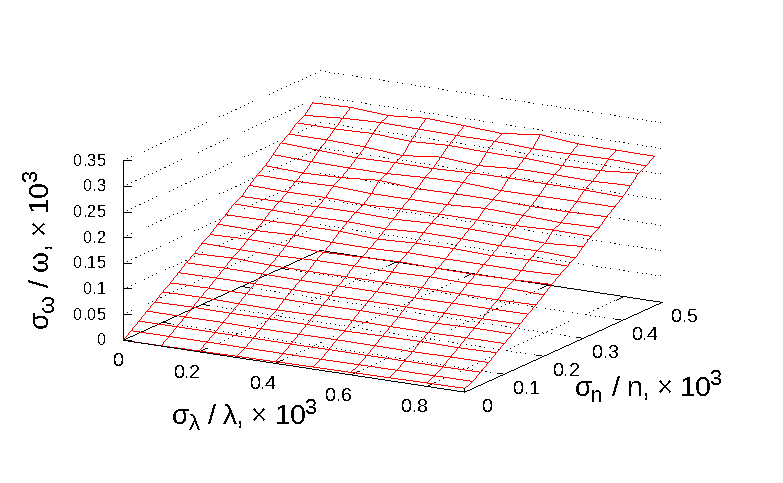
\includegraphics[scale=0.4]{figs/even/p1.txt_coeff0.dat.eps} & 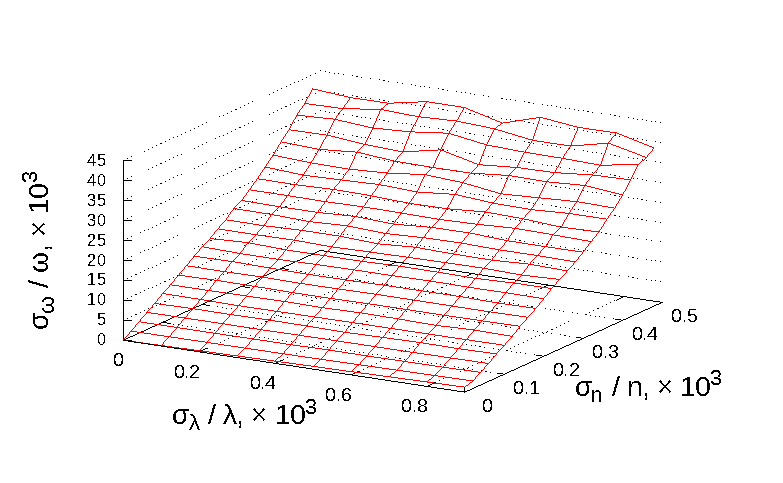
\includegraphics[scale=0.4]{figs/even/p1.txt_coeff1.dat.eps} & 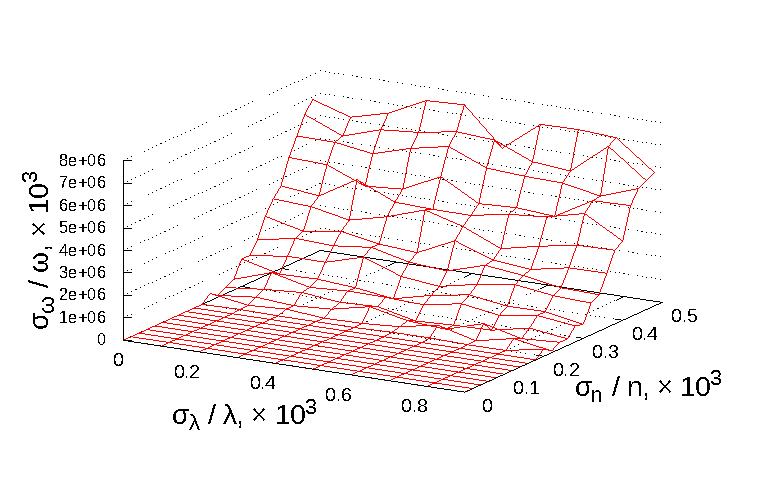
\includegraphics[scale=0.4]{figs/even/p1.txt_coeff2.dat.eps} \\
	\begin{rotate}{90}Polymer 2\end{rotate} &	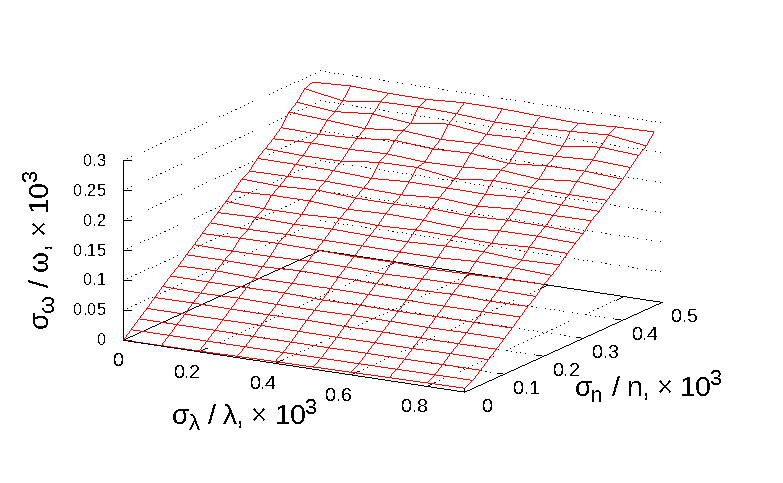
\includegraphics[scale=0.4]{figs/even/p2.txt_coeff0.dat.eps} & 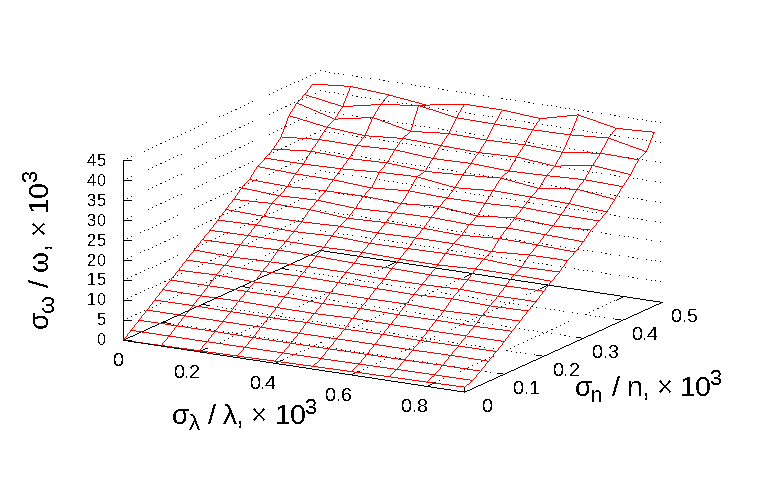
\includegraphics[scale=0.4]{figs/even/p2.txt_coeff1.dat.eps} & 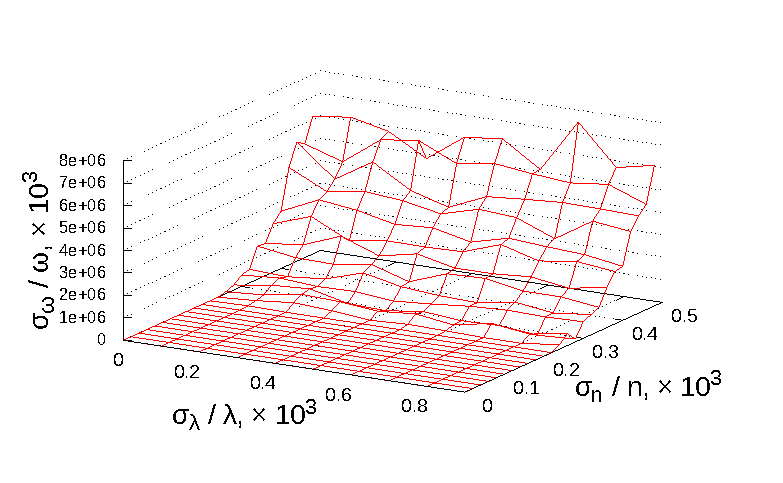
\includegraphics[scale=0.4]{figs/even/p2.txt_coeff2.dat.eps}
  \end{tabular}
  \label{tabl:res_even}
\end{table}

\begin{table}[h]
  \centering
  \footnotesize
  \caption{Coefficients of model \eqref{eq:res_0} and their relative residual.}
  \begin{tabular}{l | c | c | c | c}
				& $\omega_1$				& $\omega_2$				& $\omega_3$				& MSE	\\ \hline
    Polymer 1	& 1.34946				& 3558.95				& 1924.33				& $2.2 \cdot 10^{-8}$		\\
    Polymer 2	& 1.34047				& 3118.84				& 1578.59				& $1.4 \cdot 10^{-8}$		\\
	Residual		& $6.71 \cdot 10^{-3}$	& $1.41 \cdot 10^{-1}$	& $2.2 \cdot 10^{-1}$	&	\\
  \end{tabular}
  \label{tabl:res_even_coeffs}
\end{table}

\begin{table}[h]
  \centering
  \footnotesize
  \caption{Standard deviation of \eqref{eq:res_0} parameters for the first polymer for selected noise parameters.}
  \begin{tabular}{l | c | c | c}
	$\omega_i$	& $\frac{\sigma_{\lambda}}{\lambda} = 2 \cdot 10^{-4}; \frac{\sigma_n}{n} = 2 \cdot 10^{-5}$	& $ \frac{\sigma_{\lambda}}{\lambda} = 6 \cdot 10^{-4}; \frac{\sigma_n}{n} = 6 \cdot 10^{-5} $	& $ \frac{\sigma_{\lambda}}{\lambda} = 9 \cdot 10^{-4}; \frac{\sigma_n}{n} = 2 \cdot 10^{-4} $ \\ \hline
	1		& $1.22 \cdot 10^{-5}$																			& $ 3.59 \cdot 10^{-5} $																		& $ 1.19 \cdot 10^{-4} $		\\
	2		& $1.48 \cdot 10^{-3}$																			& $ 4.38 \cdot 10^{-3} $																		& $ 1.44 \cdot 10^{-2} $		\\
  \end{tabular}
  \label{tabl:res_even_stddev}
\end{table}

The graphs show that the wavelength measurement error does not significantly affect
first and second parameters in the region of interest. At the same time, their standard deviation
depends on the standard deviation of the refraction index almost linearly.

These results can be interpreted in the following way: during experiment planning most attention
should be paid to maximizing the certainity in measuring the refraction index, while the wavelength
can be measured quite inaccurately with errors up to few nanometers. Moreover, the suggested method
directly shows how the parameters error depends on the measurement errors of different variables.

It is fundamentally important that the standard deviation of the parameters of the model \eqref{eq:res_0}
are considerably smaller than the difference between the parameters for two polymers (as shown
by tables \ref{tabl:res_even_coeffs} and \ref{tabl:res_even_stddev}), which means that the polymers
can be separated by such measurements even with an imprecise refractometer.

\paragraph{Stability of the overfitted model.}

The stability of model \eqref{eq:res_incorrect} is studied analogously. Standard deviation
graphs for the first three parameters are shown in table \ref{tabl:res_incorrect}.

\begin{table}[h]
  \centering
  \footnotesize
  \caption{Standard deviation for \eqref{eq:res_incorrect}.}
  \begin{tabular}{l | c c c}
	  & $\omega_1$ & $\omega_2$ & $\omega_3$ \\ \hline
	\begin{rotate}{90}Polymer 1\end{rotate} &	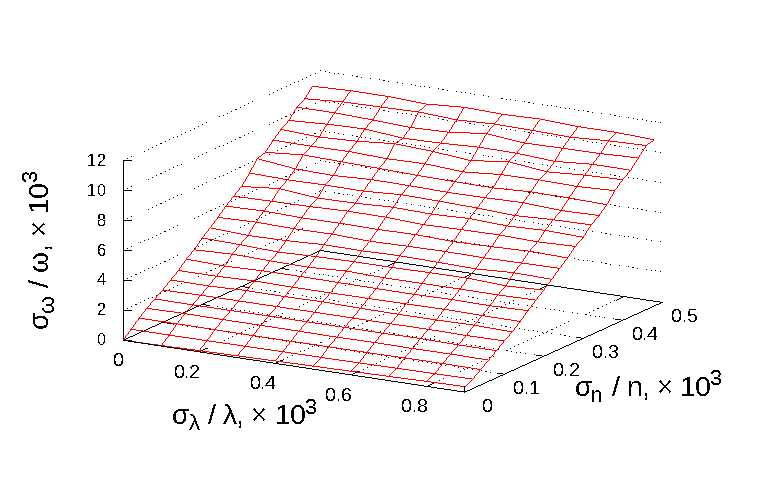
\includegraphics[scale=0.4]{figs/all/p1.txt_coeff0.dat.eps} & 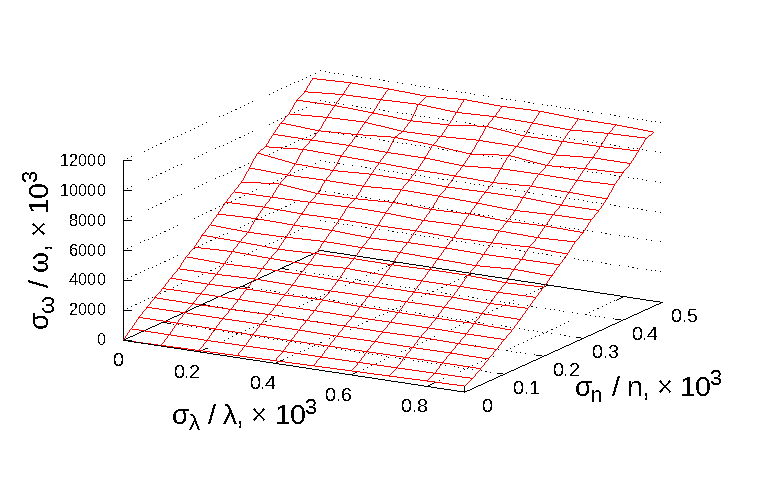
\includegraphics[scale=0.4]{figs/all/p1.txt_coeff1.dat.eps} & 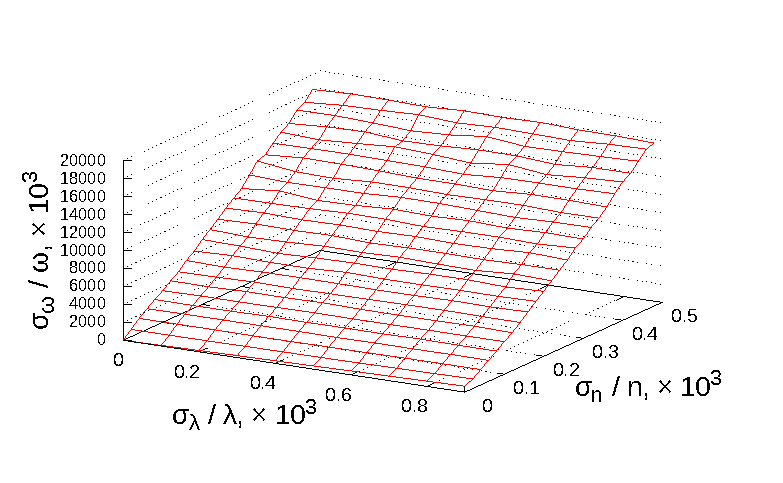
\includegraphics[scale=0.4]{figs/all/p1.txt_coeff2.dat.eps} \\
	\begin{rotate}{90}Polymer 2\end{rotate} &	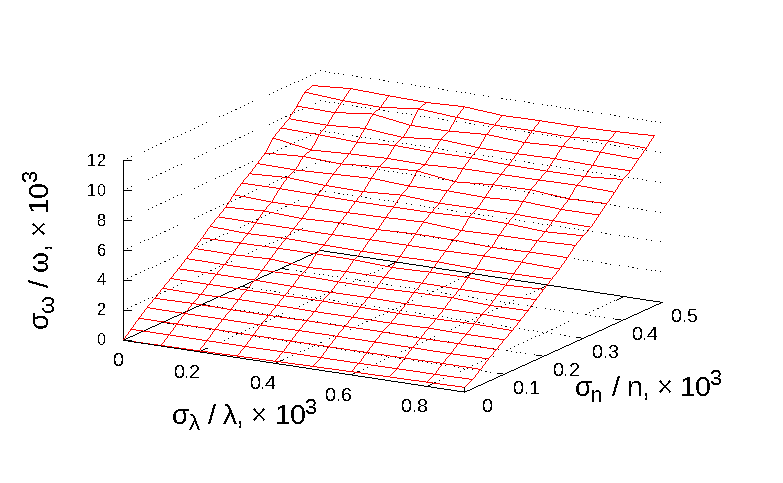
\includegraphics[scale=0.4]{figs/all/p2.txt_coeff0.dat.eps} & 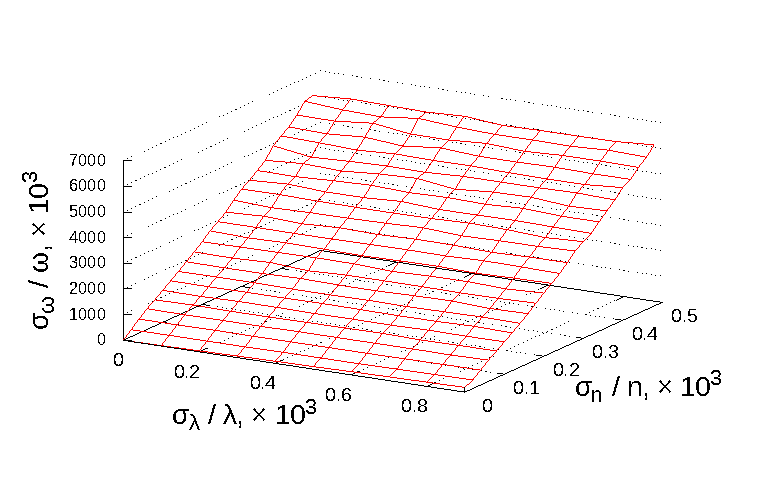
\includegraphics[scale=0.4]{figs/all/p2.txt_coeff1.dat.eps} & 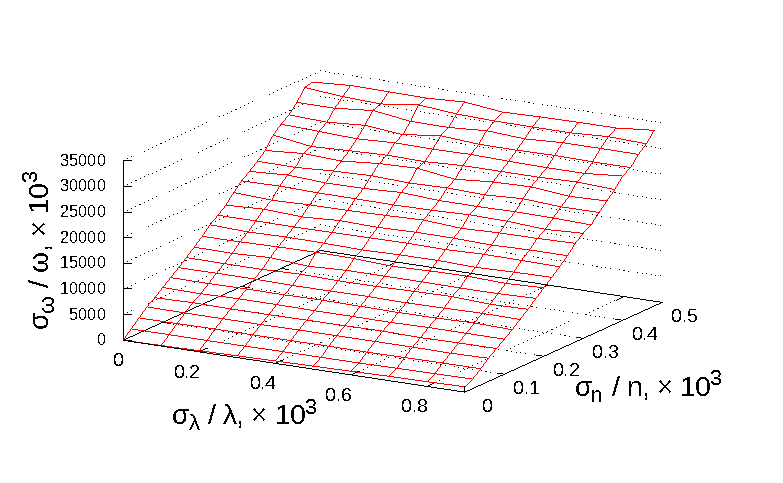
\includegraphics[scale=0.4]{figs/all/p2.txt_coeff2.dat.eps}
  \end{tabular}
  \label{tabl:res_incorrect}
\end{table}

The graphs show that standard deviation values for \eqref{eq:res_incorrect} are considerably higher
than the corresponding ones for \eqref{eq:res_0}. Particularly the second, third and fourth
parameters have standard deviation orders of magnitude higher than their corresponding values.

These results may be a sign of overfitting, and that the resulting model can't be used to
describe the physical process, and can not be used to separate two polymers in their mixture.

\section{Convergence to the linear case.}

The case of linear regression is considered:
\[
  y = ax + b.
\]
Taking the measurement errors into account:
\[
  y_i = ax_i + b + \xi_i \mid i \in \{ 1, \dots, n \},
\]
where the errors $\xi_i$ are independent, and $E(\xi_i) = 0; D(\xi_i) = \sigma^2$ \citep{Vatunin05_en}.
In other words, the error doesn't depend on the measurement, and the independent variable
is measured precisely.

According to \citep{Vatunin05_en} for the following presentation:
\[
  y_i = a(x_i - \overline{x}) + b + \xi_i \mid i \in \{ 1, \dots, n \},
\]
$a$ and $b$ are independent normally distributed random variables, and
their dispersions can be exactly calculated:
\begin{equation}
  \label{eq:classic_da}
  D(a) = \frac{\sigma^2}{\sum_{i = 1}^n (x_i - \overline{x})^2}.
\end{equation}
\begin{equation}
  \label{eq:classic_db}
  D(b) = \frac{\sigma^2}{n}.
\end{equation}

Next the results obtained by the proposed method are compared to the ones resulting
from\eqref{eq:classic_da} and \eqref{eq:classic_db}. The relative difference
between these values and empiric standard deviations is considered as a function of
number of iterations $N$:
\[
  \delta_1 = \frac{| \overline{\sigma}_a^2 - D(a) |}{D(a)},
\]
\[
  \delta_2 = \frac{| \overline{\sigma}_b^2 - D(b) |}{D(b)}.
\]

Corresponding graphs for the function $y = 2x + 1 + \xi_i$ with $x \in [0; 10]$,
$n = 10$ samples and $D(\xi_i) = 10$ are shown on fig. \ref{fig:classic_var10_n10}.
Particularly, the fig. \ref{fig:classic_var10_n10_begin} shows the initial part of the
graph for $N$ smaller than $5 \cdot 10^5$, the fig. \ref{fig:classic_var10_n10_middle}
shows the part for $N$ between $5 \cdot 10^5$ and $10^7$, and fig.
\ref{fig:classic_var10_n10_end} represents the convergence on big $N$ (from $10^7$ to $10^8$).

Analogous graphs are also shown for $n = 10$ and $D(\xi_i) = 1$, and $n = 50$ and $D(\xi_i) = 1$,
on fig. \ref{fig:classic_var1_n10} and \ref{fig:classic_var1_n50} respectively.

The graphs show that the relative difference stabilizes around $(1.5 \div 3) \cdot 10^6$
iterations and doesn't explicit dependence on the number of samples or standard
deviation of the error. The resulting relative difference is close to zero, but is
not equal to it probably to rounding errors and other similar computational effects.

\begin{figure}[h!]
  \begin{subfigure}[b]{0.3\textwidth}
    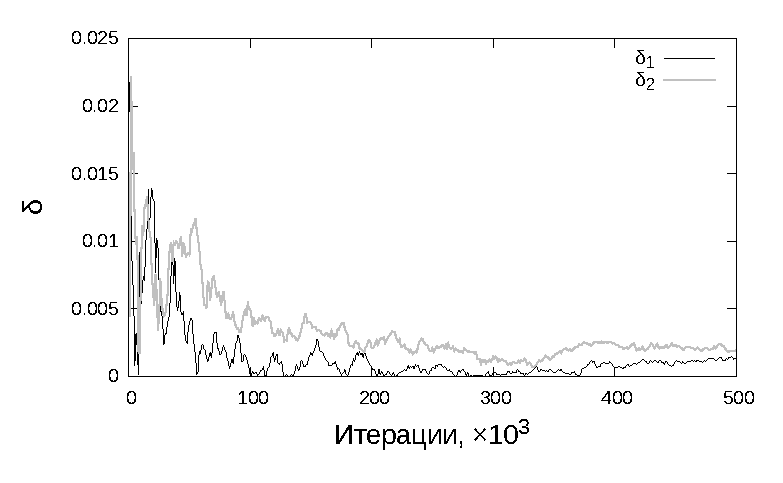
\includegraphics[width=\textwidth]{figs/classic/linear_log_1x_2_samples_10_variance_10_norm.log_0_500.eps}
    \caption{$N \in [0;~5 \cdot 10^5]$}
    \label{fig:classic_var10_n10_begin}
  \end{subfigure}
  \begin{subfigure}[b]{0.3\textwidth}
    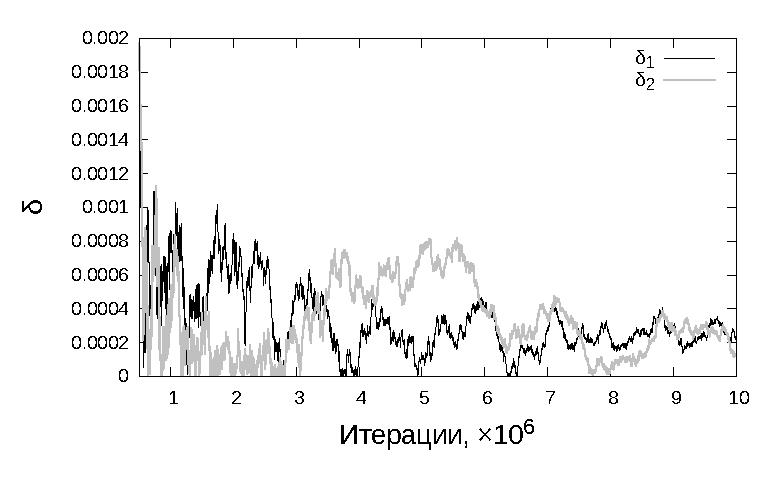
\includegraphics[width=\textwidth]{figs/classic/linear_log_1x_2_samples_10_variance_10_norm.log_500_10000.eps}
    \caption{$N \in [5 \cdot 10^5;~10^7]$}
    \label{fig:classic_var10_n10_middle}
  \end{subfigure}
  \begin{subfigure}[b]{0.3\textwidth}
    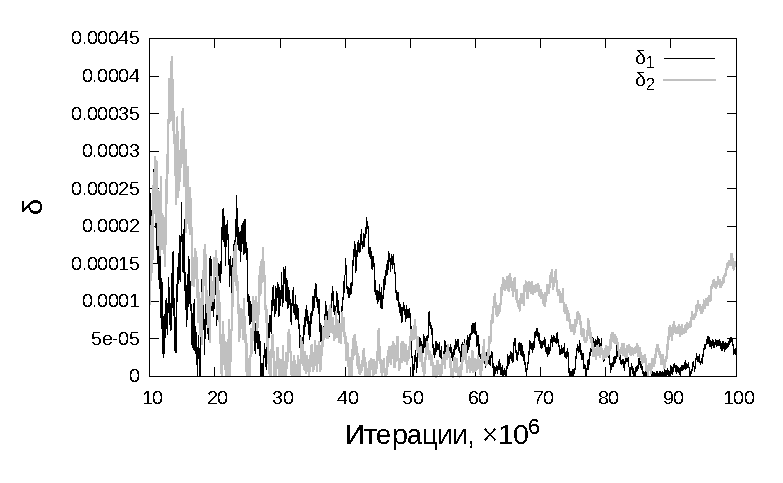
\includegraphics[width=\textwidth]{figs/classic/linear_log_1x_2_samples_10_variance_10_norm.log_end.eps}
    \caption{$N \in [10^7;~10^8]$}
    \label{fig:classic_var10_n10_end}
  \end{subfigure}
  \caption{Dependence of $\delta$ on $N$ with $D(\xi) = 10$ and $n = 10$.}
  \label{fig:classic_var10_n10}
\end{figure}

\begin{figure}[h!]
  \begin{subfigure}[b]{0.3\textwidth}
    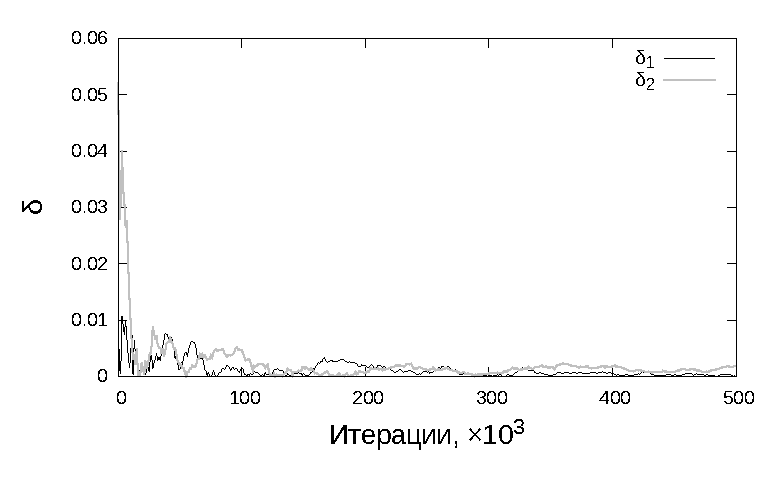
\includegraphics[width=\textwidth]{figs/classic/linear_log_1x_2_samples_10_variance_1_norm.log_0_500.eps}
    \caption{$N \in [0;~5 \cdot 10^5]$}
    \label{fig:classic_var1_n10_begin}
  \end{subfigure}
  \begin{subfigure}[b]{0.3\textwidth}
    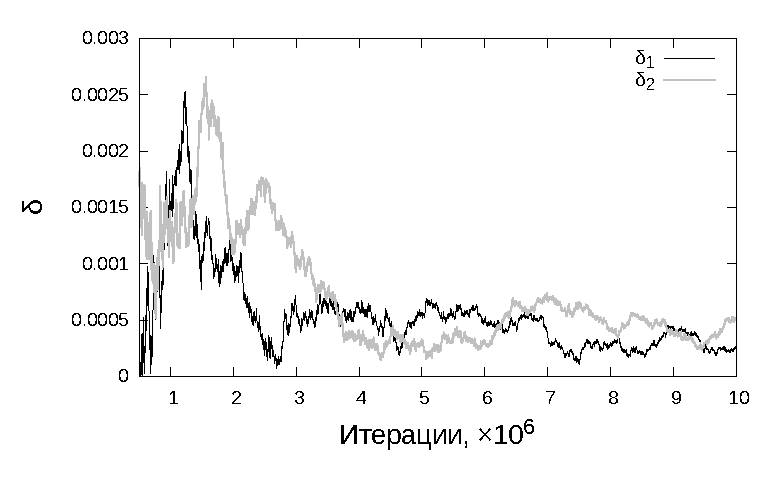
\includegraphics[width=\textwidth]{figs/classic/linear_log_1x_2_samples_10_variance_1_norm.log_500_10000.eps}
    \caption{$N \in [5 \cdot 10^5;~10^7]$}
    \label{fig:classic_var1_n10_middle}
  \end{subfigure}
  \begin{subfigure}[b]{0.3\textwidth}
    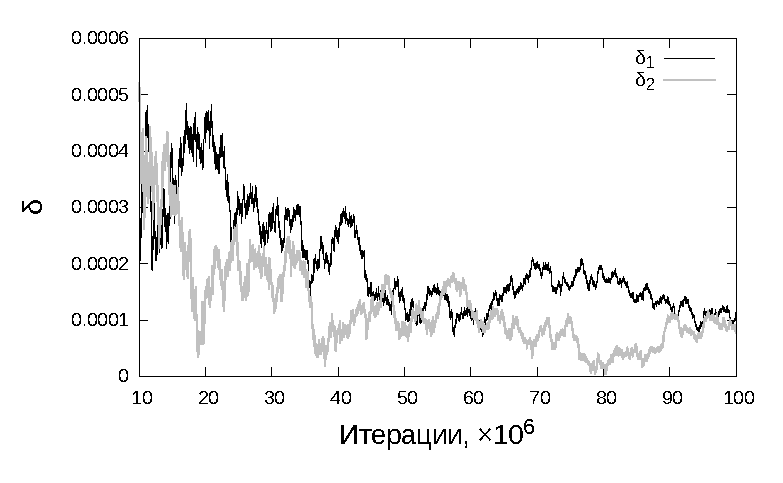
\includegraphics[width=\textwidth]{figs/classic/linear_log_1x_2_samples_10_variance_1_norm.log_end.eps}
    \caption{$N \in [10^7;~10^8]$}
    \label{fig:classic_var1_n10_end}
  \end{subfigure}
  \caption{Dependence of $\delta$ on $N$ with $D(\xi) = 1$ and $n = 10$.}
  \label{fig:classic_var1_n10}
\end{figure}

\begin{figure}[h!]
  \begin{subfigure}[b]{0.3\textwidth}
    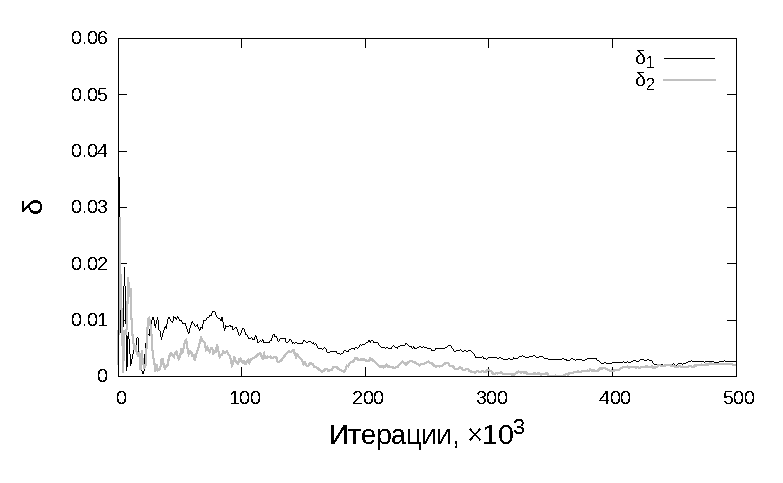
\includegraphics[width=\textwidth]{figs/classic/linear_log_1x_2_samples_50_variance_1_norm.log_0_500.eps}
    \caption{$N \in [0;~5 \cdot 10^5]$}
    \label{fig:classic_var1_n50_begin}
  \end{subfigure}
  \begin{subfigure}[b]{0.3\textwidth}
    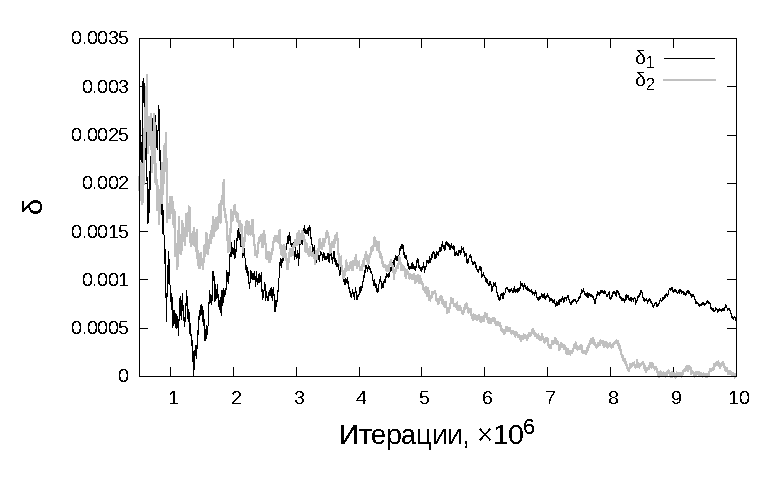
\includegraphics[width=\textwidth]{figs/classic/linear_log_1x_2_samples_50_variance_1_norm.log_500_10000.eps}
    \caption{$N \in [5 \cdot 10^5;~10^7]$}
    \label{fig:classic_var1_n50_middle}
  \end{subfigure}
  \begin{subfigure}[b]{0.3\textwidth}
    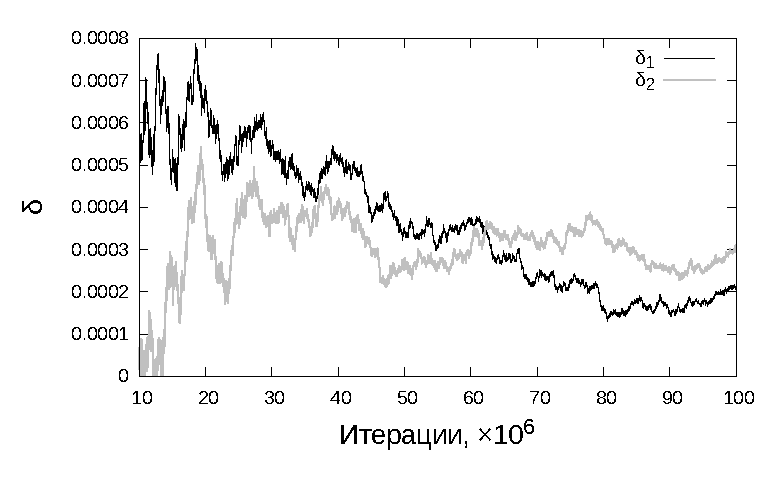
\includegraphics[width=\textwidth]{figs/classic/linear_log_1x_2_samples_50_variance_1_norm.log_end.eps}
    \caption{$N \in [10^7;~10^8]$}
    \label{fig:classic_var1_n50_end}
  \end{subfigure}
  \caption{Dependence of $\delta$ on $N$ with $D(\xi) = 1$ and $n = 50$.}
  \label{fig:classic_var1_n50}
\end{figure}

\section{Conclusion}

The algorithm proposed in \citep{Rudoy13} allows generating interpretable analytic
model describing the dependency of refraction index on the wavelength. The complexity
penalty introduced in the algorithm mitigates overfitting without resorting to methods
like crossvalidation.

Though other algorithms like SVM regression can learn models with lower mean square error,
such models are uninterpretable and prone to overfitting. Moreover, their
structural parameters need to be estimated according to, for example,
cross-validation, while the proposed method's hyperparameters can be chosen directly
according to expert considerations.

The stability criteria proposed in this paper allows studying the contribution of each
term of the resulting superposition in the overall error
and the relation between measurement errors
and errors in determining the superposition parameters. Particularly, the offered method
also allows detecting which components of feature vectors are the least susceptible to
noise in the learning data. Moreover, expertly correct models tend to be more stable
than incorrect ones.

\FloatBarrier

%\bibliographystyle{babunsrt-lf}
%\bibliographystyle{babunsrt}
%\bibliographystyle{unsrt}
\bibliography{bibliography}

\end{document}
